\documentclass[12pt,letterpaper,fleqn]{article}

%       amslatex provides nice math extensions for typesetting mathematics
\usepackage{amsmath}
\usepackage{amsfonts}
\usepackage{tmmaths}
\usepackage{sympytex}

%       pstricks provides powerful environments for incorporating postscript into a
%       TeX/LaTeX document. You must have a postscript printer and a package like
%       dvips to convert the DVI file to a PS file.
%\usepackage{pst-all}
%\usepackage{pstricks,pst-plot}
%\usepackage{pst-coil,pst-node}

%  This package provides native tex support for numbered grids. The syntax is:
%  \graphpaper[spc](x_lowleft,y_lowleft)(x_upperright,y_upperright)

%\usepackage{graphpap}
%\usepackage{float}

%  The package below must be initialized with "\initfloatingfigs" immediately after the
%  "\begin{document} command.
%\usepackage{floatfig}

\usepackage{graphicx}
\graphicspath{{i:/mytex/graphics}}
\DeclareGraphicsExtensions{.ps,.eps}

%       tst is a package for the creation of exams, quizzes and tests. the include
%       file mathstuf (see below) provides many abbreviations for these environments.
%\usepackage{tst}

%       epsfig is a package which provides for the inclusion of Encapsulated PostScript
%       files in a document.
%\usepackage{epsfig}
%\usepackage{epic,eepic}
\include{mathstuf}
\usepackage[total={7.25in,10in},top=0.25in,left=0.75in,includehead]{geometry}
\usepackage{fancyhdr}
\pagestyle{fancy}
\lhead{Math 253}
\rhead{\large Name\makebox[2in]{\hrulefill}}
\chead{\LARGE Exploration 1}
%\lfoot{\today}
\cfoot{}
%\rfoot{\thepage}
\renewcommand{\headrulewidth}{0.4pt}
\renewcommand{\footrulewidth}{0.4pt}
\setlength{\parindent}{0pt}
\setlength{\parskip}{2ex}

\newcounter{tf}[enumi]
\newenvironment{tf}[0]{\begin{list}%
{\alph{tf}. \makebox[5em]{True\hfill False}}%
{\usecounter{tf}\setlength{\labelwidth}{7em}%
\setlength{\leftmargin}{3.5cm}%
\setlength{\labelsep}{1cm}}}%
{\end{list}}

%\usepackage{epic,eepic}
\newcommand{\numline}{%
%\newcounter{mark}%
%\setcounter{mark}{-1}%
\setlength{\unitlength}{0.1in}%
\begin{picture}(0,0)%
\thicklines%
\put(0,0){\line(1,0){60}}%
\multiput(0,0)(10,0){7}{\line(0,-1){1}%
\makebox(0,-1.5)[t]{\arabic{mark}}\stepcounter{mark}}%
%
\thinlines%
\multiput(0,0)(5,0){12}{\line(0,-1){0.5}}%
\multiput(0,0)(1,0){60}{\line(0,-1){0.3}}%
%\put(-5,265){\makebox(0,0)[l]{{\bf cm}}}%
\end{picture}}%

\newcommand{\ds}{\displaystyle}
\usepackage{amsfonts}


\let\oldhat\hat
\renewcommand{\hat}[1]{\oldhat{\boldsymbol{\mathbf{#1}}}}
\newcommand{\lv}[1]{\ensuremath{\langle #1 \rangle}}
\renewcommand{\i}{\ensuremath{\hat{\imath}}}
\renewcommand{\j}{\ensuremath{\hat{\jmath}}}
\renewcommand{\k}{\ensuremath{\mathbf{\oldhat{k}}}}
\newcommand{\ora}[1]{\ensuremath{\overrightarrow{#1}}}
\renewcommand{\vec}[1]{\ensuremath{\mathbf{#1}}}
\renewcommand{\v}[1]{\ensuremath{\vec{#1}}}
\newcommand{\abs}[1]{\ensuremath{\lvert #1 \rvert}}

\usepackage{tabularx}
\usepackage{paralist}
\newcommand{\red}[1]{\textcolor{red}{#1}}
\newcommand{\blue}[1]{\textcolor{blue}{#1}}
% \newcommand{\ans}[1]{\quad\fbox{answer: \red{#1}}}
\newcommand{\ans}[1]{\mbox{{\bf Ans:} \blue{#1}}}
\newcommand{\dd}[2][]{\ensuremath{\frac{\text{d}#1}{\text{d}#2}}}
\newcommand{\eval}[2]{\ensuremath{\left.#1\right|_{#2}}}


\begin{document}
\begin{enumerate}
 \item Describe three different perspectives of the concept of ``vector''; The physics student, computer science student and mathematics student perspectives.
 \item An object moves along the $x$ axis. Its velocity is positive if it moves to the right. It's velocity is negative if it moves to the left. At time $t = 0$ the object is at the origin. The graph below shows the velocity of the object during 30 seconds of motion. What is the displacement of the object at the end of 30 seconds?
       \begin{figure}[!htb]
        \centering
        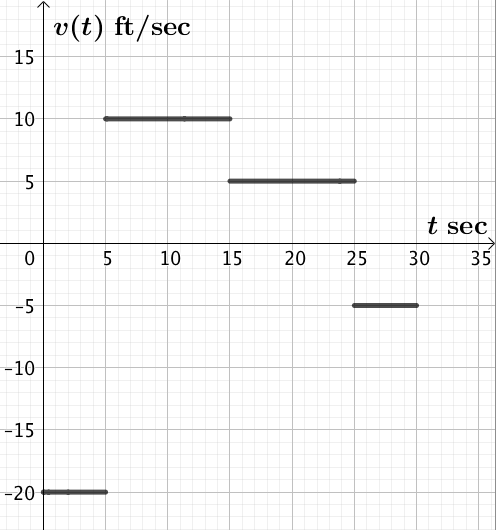
\includegraphics[width=3in]{img/velocity.png}
        % \caption{}
        % \label{}
       \end{figure}
 \item Below is the graph of the speed of the object during 30 seconds of motion. What is the total distance the object moved at the end of 30 seconds?
       \begin{figure}[!htb]
        \centering
        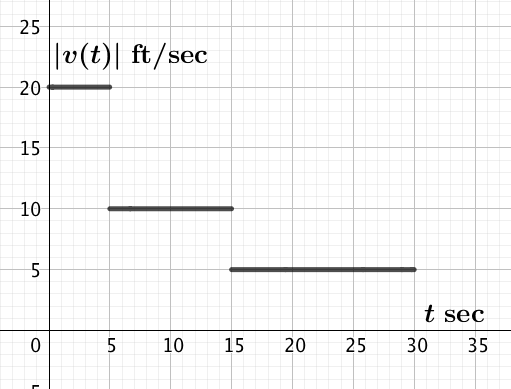
\includegraphics[width=3in]{img/speed.png}
        % \caption{}
        % \label{}
       \end{figure}
\end{enumerate}
\end{document}
